% Recommended papers: Tools and datasets for mining libre software repositories
%			The promises and perils of mining git
%
%
%
%
%

% $Id: slides.tex 4228 2006-06-21 21:55:12Z jjamor $
%
%
% Compilar a .pdf con LaTeX (pdflatex)
% Es necesario instalar Beamer (paquete latex-beamer en Debian)
%

%
% Gráficos:
% Los gráficos pueden suministrarse en PNG, JPG, TIF, PDF, MPS
% Los EPS deben convertirse a PDF (usar epstopdf)
%

\documentclass{beamer}
\usetheme{Warsaw}
\usebackgroundtemplate{
\includegraphics[width=\paperwidth]{format/libresoft-bg.png}}
\usepackage[spanish]{babel}
\usepackage[utf8]{inputenc}
\usepackage{graphics}
\usepackage{amssymb} % Simbolos matematicos
\usepackage{url}

%\definecolor{libresoftgreen}{RGB}{162,190,43}
%\definecolor{libresoftblue}{RGB}{0,98,143}

%\setbeamercolor{titlelike}{bg=libresoftgreen}

%% Metadatos del PDF.
\hypersetup{
  pdftitle={FLOSS Data Sources and Metrics},
  pdfauthor={Daniel Izquierdo},
  pdfcreator={GSyC/Libresoft},
  pdfproducer=PDFLaTeX,
  pdfsubject={nn},
}
%%


\AtBeginSection[]
{
  \begin{frame}<presentation>
    \frametitle{Index}
    \tableofcontents[current]
  \end{frame}
}


\begin{document}

\title{Introduction to FLOSS Data Sources}
\subtitle{Master on Free Software}
\institute{\\dizquierdo@libresoft.es\\
GSyC/Libresoft}
\author{Daniel Izquierdo}
\date{\today}

\frame{
\maketitle
\begin{center}

\includegraphics[width=6cm]{format/gsyc-urjc}
\end{center}
}


% Si el titulo o el autor se quieren acortar para los pies de página
% se pueden redefinir aquí:
%\title{Titulo corto}
%\author{Autores abreviado}


%% LICENCIA DE REDISTRIBUCION DE LAS TRANSPAS
\frame{
~
\vspace{4cm}

\begin{flushright}
{\tiny
(cc) 2011 Daniel Izquierdo. \\
Some rights reserved. This document is distributed under the Creative \\
            Commons Attribution-ShareAlike 3.0 licence, available in \\
            http://creativecommons.org/licenses/by-sa/3.0/

%  Este documento (o uno muy similar) está disponible en \\
%  \url{http://gsyc.escet.urjc.es/~jjamor/}
}
\end{flushright}
}
%%

%%%%%%
%Transpas separadas por \begin{frame}
%%%%%%%%%%%%%%%%%%%%%%%%\end{frame}

\section{Introduction}

\begin{frame}
\frametitle{Data sources}
\begin{itemize}
\item Source code management system
\item Mailing lists
\item Bug tracking system
\item Source code
\end{itemize}
\end{frame}

%%%%%%%%%%%%%%%%%%%%%%%%%%%%%%%%%%%%%%%%%%%%%%%%%%%%%%%%%%%%%%

\begin{frame}
 \frametitle{Data sources}
 \begin{itemize}
 \item What type of metrics can we retrieve from them?
 \end{itemize}
\end{frame}

%%%%%%%%%%%%%%%%%%%%%%%%%%%%%%%%%%%%%%%%%%%%%%%%%%%%%%%%%%%%%%


\section{Metrics}
\begin{frame}
 \frametitle{SCM: main attributes}
 \begin{itemize}
  
  \item Per commit:
   \begin{itemize}
    \item Owner of the change: committer or author
    \item Date of commit
    \item Files \emph{touched}
    \item Message left by the committer or author
    \item Lines involved in the changes
   \end{itemize} 
 \end{itemize}
\end{frame}

%%%%%%%%%%%%%%%%%%%%%%%%%%%%%%%%%%%%%%%%%%%%%%%%%%%%%%%%%%%%%%

\begin{frame}
 \frametitle{SCM: main metrics}
 \begin{itemize}
 \item Regarding to the size of the project or community:
   \begin{itemize}
    \item Number of commits
    \item Number of committers/authors
    \item Number of files \emph{touched}
    \item Number of lines \emph{touched}
    \item Usual programming language used (based on the file path)
    \item Others...
   \end{itemize}
 \end{itemize}
\end{frame}



\begin{frame}
 \frametitle{SCM: main metrics}
 \begin{itemize}
 \item Workload adequacy
  \begin{itemize}
  \item Average number of commits per committer/author
  \item Average number of files/lines touched by committer/author
  \item Territoriality: number of files only handled by just one developer
  \end{itemize}
 \end{itemize}


\end{frame}



\begin{frame}
 \frametitle{SCM: main metrics}
 \begin{itemize}
 \item Distribution of effort:
  \begin{itemize}
    \item Distribution of commits per developers (generally following a 20\% - 80\% distribution)
    \item Distribution of modules or areas of the source code by developer
    \item Others...
  \end{itemize}
 \end{itemize}
\end{frame}


\begin{frame}
 \frametitle{SCM: main metrics}
 \begin{itemize}
 \item Social network analysis
  \begin{itemize}
    \item Creation of networks based on the type of action (e.g.: two developers working in the same file, people working in the same programming language)
    \item Betweeness: interesting people with a high know-how of the community (usually found as heading two different networks of people)
  \end{itemize}
 \end{itemize}
\end{frame}


\begin{frame}
 \frametitle{SCM: main metrics}
 \begin{itemize}
 \item Evolutionary studies
  \begin{itemize}
  \item Evolution in number of new people coming to the community (regeneration of developers)
  \item Evolution in the number of fixing commits (data left by developers in the log message)
  \item Evolution in number of commits (is the community growing in activity?)
  \end{itemize}
 \end{itemize}


\end{frame}



\begin{frame}
 \frametitle{Mailing list: main metrics}
 \begin{itemize}
  \item Size of the community:
    \begin{itemize}
     \item Number of unique posters in the mailing lists
     \item Number of users posting
     \item Number of developers posting
     \item Number of mailing lists (specific mailing lists for developers, users, per language, etc)
    \end{itemize}
 \end{itemize}
\end{frame}



\begin{frame}
 \frametitle{Mailing list: main metrics}
 \begin{itemize}
  \item Workload adequacy: 
  \begin{itemize}
    \item How many developers are interacting with end users?
    \item Number of e-mails per developer / per user
    \item Number of e-mails per mailing list
  \end{itemize}

 \end{itemize}

\end{frame}


\begin{frame}
 \frametitle{Mailing lists: main metrics}
 \begin{itemize}
 \item Social network analysis:
  \begin{itemize}
   \item Similar to metrics found in the SCM
   \item Detection of important people not registered in the SCM (lawyers)
  \end{itemize}
 \end{itemize}
\end{frame}


\begin{frame}
 \frametitle{Mailing lists: main metrics}
 \begin{itemize}
 \item Evolutionary analysis:
  \begin{itemize}
   \item Evolution in the number of new people posting new e-mails
   \item Evolution in the general activity in the Mailing lists
  \end{itemize}
 \end{itemize}
\end{frame}



\begin{frame}
 \frametitle{BTS: main metrics}
 \begin{itemize}
 \item Size metrics:
  \begin{itemize}
   \item Number of bugs
   \item Number of open bugs
   \item Number of closed bugs
   \item Number of developers fixing bugs
   \item Number of users reporting bugs
   \item Number of developers reporting bugs
  \end{itemize}
 \end{itemize}
\end{frame}


\begin{frame}
 \frametitle{BTS: main metrics}
 \begin{itemize}
 \item Workload adequacy:
  \begin{itemize}
   \item Average number of bugs fixed per developer
   \item Average number of bugs remaining open per developer
  \end{itemize}
 \end{itemize}
\end{frame}




\begin{frame}
 \frametitle{Source code: main metrics}
 \begin{itemize}
 \item Size adequacy:
  \begin{itemize}
   \item Number of lines
   \item Number of files
   \item Types of programming languages
   \item Types of files (source code, translation, images, etc...)
   \item Number of lines per file
  \end{itemize}
 \end{itemize}
\end{frame}





\begin{frame}
\frametitle{Source code: main metrics}
\begin{center}
\begin{figure}
 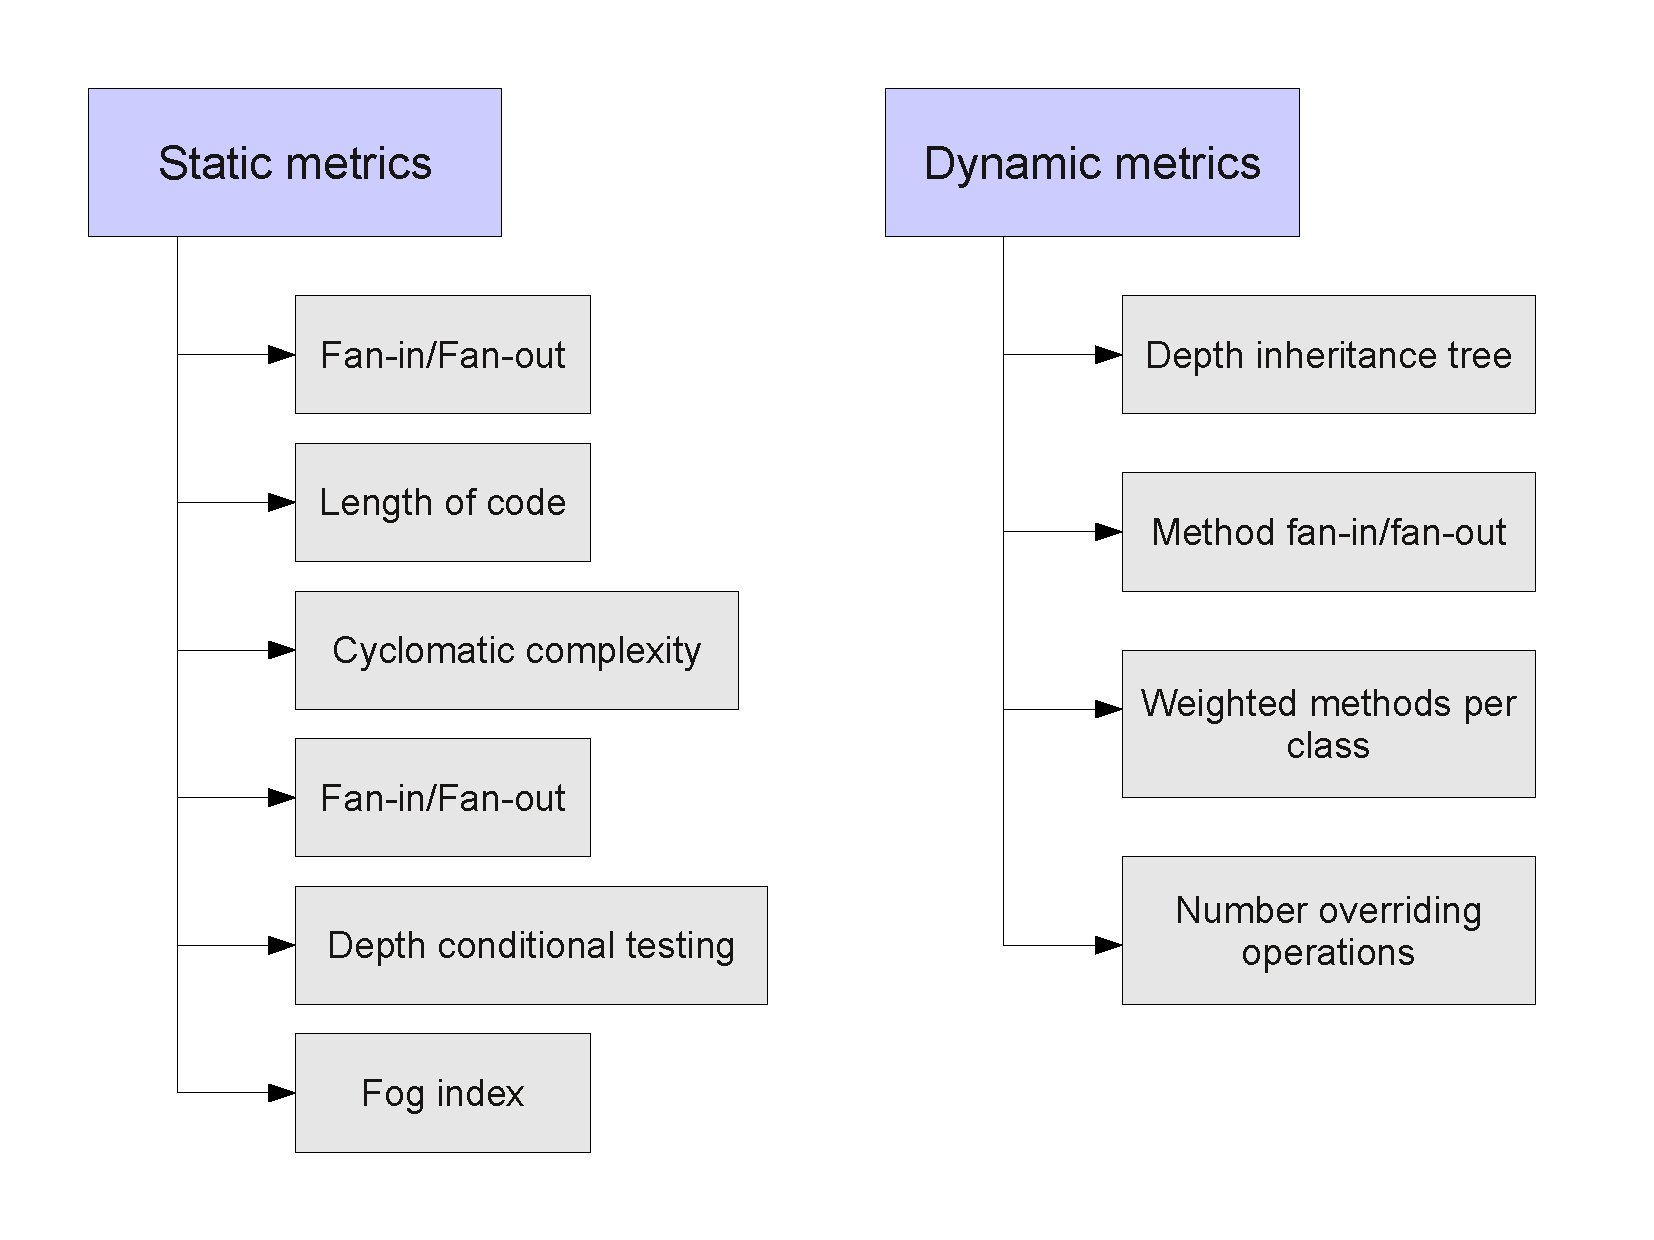
\includegraphics[height=7cm]{figs/quality-product-metrics.pdf}
\end{figure}
\end{center}
\end{frame}

%%%%%%%%%%%%%%%%%%%%%%%%%%%%%%%%%%%%%%%%%%%%%%%%%%%%%%%%%%%%%%

\begin{frame}
 \frametitle{Source code: main metrics}
 \begin{itemize}
 \item Static metrics:
 \begin{itemize}
  \item \textit{Fan-in/Fan-out}: Number of functions or methods that call some other
function or method (complexity, connascence).
  \item \textit{Length of code}: Size of program. SLOC (LOC or LLOC).
  \item \textit{Cyclomatic complexity}: Metric for control complexity of software.
  \item \textit{Length of identifiers}: Average length of identifiers used in a program.
Supposedly, the longer the ID, the better for readability and maintenance of code.
  \item \textit{Depth of conditional nesting}: Deeply nested statements are harder to be grasped.
  \item \textit{Fog index}: Average length of words and sentences in documents.
 \end{itemize}

 \end{itemize}
\end{frame}


\begin{frame}
 \frametitle{Source code: main metrics}
 \begin{itemize}
 \item Dynamic metrics:
 \begin{itemize}
  \item \textit{Depth of inheritance tree}: Number of discrete levels in the tree of
classes (OOP). The deeper the tree, the more complex the desgin.
  \item \textit{Method fan-in/fan-out}: Distinction between origin of calls to other
methods (from object or from external methods).
  \item \textit{Weighted methods per class}: Number of methods included in a class, weighted complexity
of every method. Too complex classes are difficult as for understanding and maintenance.
  \item \textit{Number of overriding operations}: Operations overridden in sub-classes. The higher this
number, the less appropriate may be the super-class.
 \end{itemize}

 \end{itemize}
\end{frame}



\begin{frame}
 \frametitle{Source code: main metrics}
 \begin{itemize}
 \item Evolutionary studies:
  \begin{itemize}
   \item Evolution of the number of lines
   \item Clones detection (are parts of the source code being moved to another areas?)
   \item Evolution of the architecture
   \item Others...
  \end{itemize}
 \end{itemize}
\end{frame}


\section{Conclusions}

\begin{frame}
 \frametitle{Using metrics}
 \begin{itemize}
 \item Metrics are providing objective results, however general conclusions
 should be inferred from those.

 \item Thus, human interpretation is needed.

 \item Benchmarks could be created in order to have a comparison model

 \item With that benchmark, you will be able to compare the current situation of the 
 assessed project with others 

 

 \end{itemize}

\end{frame}


\section{References}

\begin{frame}
 \frametitle{References}
 \begin{itemize}
 \item Producing OSS by \textit{Karl Fogel}
 \item Tools and datasets for mining libre software repositories, by
 \textit{Gregorio Robles, Jes\'us M. Gonz\'alez-Barahona, Daniel Izquierdo-Cort\'azar and Israel Herraiz}
 \item Metrics and Models in Software Quality Engineering
 \textit{by Stephen H. Kan}
 \end{itemize}

\end{frame}

\end{document}